%%%%%%%%%%%%%%%%%%%%%%%%%%%%%%%%%%%%%%%%%
% Stylish Article
% LaTeX Template
% Version 2.2 (2020-10-22)
%
% This template has been downloaded from:
% http://www.LaTeXTemplates.com
%
% Original author:
% Mathias Legrand (legrand.mathias@gmail.com) 
% With extensive modifications by:
% Vel (vel@latextemplates.com)
%
% License:
% CC BY-NC-SA 3.0 (http://creativecommons.org/licenses/by-nc-sa/3.0/)
%
%%%%%%%%%%%%%%%%%%%%%%%%%%%%%%%%%%%%%%%%%

%----------------------------------------------------------------------------------------
%	PACKAGES AND OTHER DOCUMENT CONFIGURATIONS
%----------------------------------------------------------------------------------------

\documentclass[fleqn,10pt]{SelfArx} % Document font size and equations flushed left
\usepackage[english]{babel} % Specify a different language here - english by default
\usepackage{graphicx}


%----------------------------------------------------------------------------------------
%	COLUMNS
%----------------------------------------------------------------------------------------

\setlength{\columnsep}{0.55cm} % Distance between the two columns of text
\setlength{\fboxrule}{0.75pt} % Width of the border around the abstract

%----------------------------------------------------------------------------------------
%	COLORS
%----------------------------------------------------------------------------------------

\definecolor{color1}{RGB}{0,0,90} % Color of the article title and sections
\definecolor{color2}{RGB}{0,20,20} % Color of the boxes behind the abstract and headings

%----------------------------------------------------------------------------------------
%	HYPERLINKS
%----------------------------------------------------------------------------------------

\usepackage{hyperref} % Required for hyperlinks

\hypersetup{
	hidelinks,
	colorlinks,
	breaklinks=true,
	urlcolor=color2,
	citecolor=color1,
	linkcolor=color1,
	bookmarksopen=false,
	pdftitle={Title},
	pdfauthor={Author},
}

%----------------------------------------------------------------------------------------
%	ARTICLE INFORMATION
%----------------------------------------------------------------------------------------

\JournalInfo{\today}
\Archive{ } % Additional notes (e.g. copyright, DOI, review/research article)

\PaperTitle{NUFORC Data Visualization on JavaScript} % Article title

\Authors{Joshua Matthew Mc Laughlin, Jonas Luca Wolter}

\Keywords{NUFORC --- p5.js --- d3.js} % Keywords - if you don't want any simply remove all the text between the curly brackets
\newcommand{\keywordname}{Keywords} % Defines the keywords heading name

%----------------------------------------------------------------------------------------
%	ABSTRACT
%----------------------------------------------------------------------------------------

\Abstract{
For the project, the dataset to be used is from an organization called NUFORC (National UFO Reporting Center) \cite{nuforc_webpage}, which takes in reports made by people around the world and investigates potential explanations of these phenomena.
The dataset contains 80,000 reports of UFO sightings from 1905 to 2014. The dataset is available on HuggingFace \cite{nuforc_dataset}.
The information contained in the data is: date, city, state, country, shape, duration, and comments.
The goal of the project is to interactively visualize data in a way that allows us to gain insights into the distribution of sightings across the world and over time, while also making sure the graphs are easy to understand and interact with. The tools to be used for the project are JavaScript libraries such as p5.js \cite{p5.js} and d3.js \cite{d3.js}, which are powerful tools for creating interactive data visualizations on the web, also allowing us to create a more immersive experience by using AR (Augmented Reality) as another visualization method.
}

%----------------------------------------------------------------------------------------

\begin{document}

\maketitle % Output the title and abstract box

\tableofcontents % Output the contents section

\thispagestyle{empty} % Removes page numbering from the first page

%----------------------------------------------------------------------------------------
%	ARTICLE CONTENTS
%----------------------------------------------------------------------------------------
\section{NUFORC}
NUFORC (National UFO Reporting Center) is an organization that collects and investigates reports of UFO sightings from around the world. 
The organization was founded in 1974 by Robert J. Gribble, and it has been collecting data on UFO sightings ever since. The data is collected through a variety of channels, including phone calls, emails, and online forms.
They also investigate potential explanations for the sightings, such as weather phenomena, aircrafts.
The dataset contains 80,000 reports of UFO sightings from 1905 to 2014. The information contained in the data is:

date, city, state, country, shape, duration, summary and an explanation text.

\newpage % Makes a new page for the rest of the content
\section{Design UX}

The idea for this data visualization is an immersive experience where the user can feel like they are in the middle of the data, being able to interact with it and explore it in a more intuitive way.
For that reason, the use of AR is a key aspect of the design, allowing the user to interact with the data in a more natural way or in intergalactic scenarios.

\begin{enumerate}[noitemsep] % [noitemsep] removes whitespace between the items for a compact look
\item Background of the page is dark, with a touch of blue, to create a mysterious and immersive atmosphere.
\item The font is in a light color, maybe a bit glowing, to contrast with the dark background and make it easier to read.
\item The graphs are big and interactive, allowing the user to explore the data in a more intuitive way. The use of AR allows the user to interact with the data in a more natural way or in intergalactic scenarios.
\end{enumerate}

Important things to consider are the accessibility of the graphs, making sure to take into account color blindness and other visual impairments, as well as making sure the graphs are easy to understand and interact with.
This includes the use of clear labels, tooltips, and other interactive elements that can help the user understand the data better.
For the design of the graphs, a consistent color scheme will be used, avoiding colors such as red and green together, or yellow for text, to make sure the elements are easy to distinguish and read.
Text should also be big enough to be read easily.

%------------------------------------------------

\newpage
\section{Visualization Ideas}
For each of the following visualizations, we first define a user story that motivates the chart, and then justify why this specific type of visualization is the most suitable choice for the underlying question.

\subsection{Calender Heatmap}
% One of the methods to analyse the data could be a calendar heatmap, to view the distribution of sightings over the years. Information to be gathered could be specific increases in sightings, correlating with historical events, or specific seasons of the year where sightings are more common. The calendar heatmap could be filtered by year.

\textbf{User Story:} \textit{As a data explorer, I want to see how UFO sightings are distributed across days and years, so that I can identify temporal patterns, seasonal effects, or anomalies that may correlate with historical events.}
\\
\textbf{Justification:} A calendar heatmap is well suited for this question because it encodes a single quantitative variable (number of sightings) on two cyclic temporal dimensions (day-of-year and year). Compared to a simple line chart, it preserves the calendar structure and allows the user to spot weekday effects, summer peaks, or specific dates of unusual activity at a glance. The colour intensity provides a pre-attentive cue, making outliers immediately visible without requiring the user to read exact numbers. Filtering by year allows a more detailed comparison between individual periods.

\begin{figure}[ht]
\centering
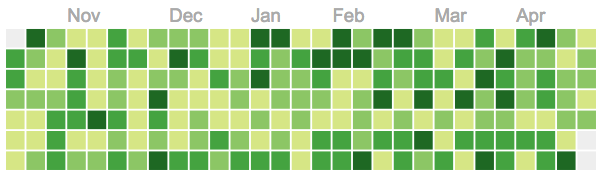
\includegraphics[width=\linewidth]{calender.png}
\caption{Example of a calendar heatmap \cite{calender_webpage}}
\label{fig:calender-heatmap}
\end{figure}

\subsection{Geographical Heatmap}

% In order to view the distribution of sightings across the world, a geographical heatmap could be used.
% This would allow us to see if there are specific areas where sightings are more common, and which countries are the main contributors.
% Here is where AR could be useful to visualize the data in a more interactive way, being able to view specific angles of the heatmap by interacting with the camera.
\textbf{User Story:} \textit{As a curious user, I want to explore the geographical distribution of UFO sightings on an interactive globe, so that I can understand which regions of the world report the most sightings and discover potential geographical hotspots.}
\\
\textbf{Justification:} The data contains an inherent spatial component (city, state, country), which makes a map-based visualization the natural choice.
Any non-spatial chart would discard this dimension. A heatmap overlay on a globe scales well to a large number of data points (80{,}000 reports) without the visual clutter that individual markers would produce.
Using a 3D globe instead of a flat projection avoids the distortions of common map projections (e.g.\ Mercator) and reinforces the global, "intergalactic" theme of the project.
The AR extension further leverages the spatial nature of the data by allowing the user to physically change the viewing angle.


\begin{figure}[ht]
\centering
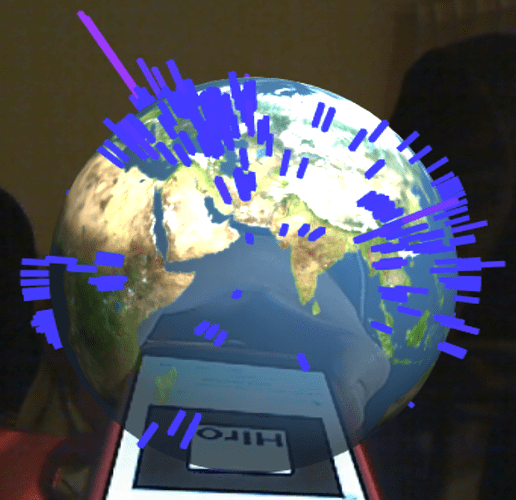
\includegraphics[width=\linewidth, height=7.5cm]{Globe.png}
\caption{Example of a geographical heatmap \cite{globe_webpage}}
\label{fig:geographical-heatmap}
\end{figure}

\newpage

\subsection{Bubble Chart}

% A bubble chart could be used to visualize the most common words used in the comments section of the reports.
% This could give us insight into the common themes and descriptions used by witnesses.
% Potentially being able to filter the bubble chart by features such as shape, duration, or location could provide more specific insights into the data.

\textbf{User Story:} \textit{As a researcher, I want to see which words and themes appear most frequently in the witness comments, so that I can quickly grasp the dominant descriptions and language patterns used by observers.}
\\
\textbf{Justification:} The summary column contains unstructured text data, which can be summarized by counting the frequency of individual words or phrases. A bubble chart encodes this information by representing each word as a circle, where the size corresponds to its frequency. This allows the user to immediately identify the most common terms without needing to read through the raw text. Compared to a bar chart, a bubble chart can display more categories in a compact space and emphasizes the relative importance of each word through size rather than length. Filtering by other features (shape, duration, location) adds an additional layer of interactivity, enabling users to explore how language varies across different contexts.

\begin{figure}[ht]
    \centering
    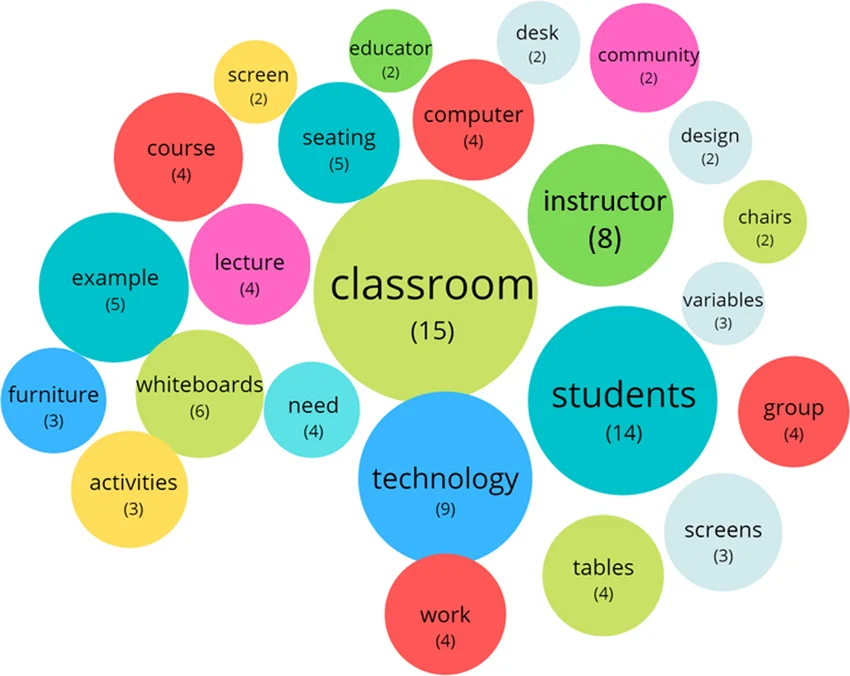
\includegraphics[width=\linewidth, height=6.5cm]{bubble.png}
    \caption{Example of a bubble chart\cite{bubble_webpage}}
    \label{fig:bubble-chart}
\end{figure}



\newpage
%------------------------------------------------

%----------------------------------------------------------------------------------------
%	REFERENCE LIST
%----------------------------------------------------------------------------------------


\bibliographystyle{unsrt}
\bibliography{sample.bib}

%----------------------------------------------------------------------------------------

\end{document}